\section{Мета роботи}
Отримання практичних навичок визначення конфігурації та основних характеристик ПЕОМ та її модулів.

\section{Хід роботи}
\subsection{Постановка задачі}
\textbf{Завдання:} визначити кількість підключених принтерів та дату створення BIOS;
перевірити, чи правильно встановлено годинник реального часу.

\subsection{Код програми}
Для виконання роботи було написано наступний скрипт:

\begin{lstlisting}[style=customc]
#include <dos.h>
#include <stdio.h>

void check_printers(void);
void check_bios_date(void);
void check_rtc(void);

// functions that checks amount of connected printers
void check_printers(void) {
    unsigned int config_word;
    unsigned int printer_count;

    config_word = *(unsigned int far *)MK_FP(0x40, 0x10);
    printf("Raw configuration word: 0x%X\n", config_word);
    printer_count = (config_word >> 14) & 0x03;

    if (printer_count > 0) {
        printf("Number of connected printers: %u\n", printer_count);
    } else {
        printf("No printers are connected.\n");
    }
}

// function that checks bios creation date
void check_bios_date() {
    char bios_date[9];
    int i;

    for (i = 0; i < 8; i++) {
        bios_date[i] = *(char far *)MK_FP(0xF000, 0xFFF5 + i);
    }
    bios_date[8] = '\0';

    printf("BIOS creation date: %s\n", bios_date);
}

int bcd_to_bin(int bcd_value) {
    return ((bcd_value >> 4) * 10) + (bcd_value & 0x0F);
}

// function that setups realtime clock
void check_rtc() {
    int seconds;
    int minutes;
    int hours;
    int day;
    int month;
    int year;

    outp(0x70, 0x00);
    seconds = bcd_to_bin(inp(0x71));
    outp(0x70, 0x02);
    minutes = bcd_to_bin(inp(0x71));
    outp(0x70, 0x04);
    hours = bcd_to_bin(inp(0x71));
    outp(0x70, 0x07);
    day = bcd_to_bin(inp(0x71));
    outp(0x70, 0x08);
    month = bcd_to_bin(inp(0x71));
    outp(0x70, 0x09);
    year = bcd_to_bin(inp(0x71));

    printf("The current hour: %02d:%02d:%02d:%02d\n", hours, minutes, seconds);
    printf("The current date: %02d/%02d/20%02d\n", day, month, year);

    if (seconds < 60 && minutes < 60 && hours < 24 && day <= 31 && month <= 12) {
        printf("Real hour year is set correctly.\n");
    } else {
        printf("Real hour year is set incorrectly.\n");
    }
}

// main function where all other functions called
int main() {
    check_printers();
    check_bios_date();
    check_rtc();
    return 0;
}
\end{lstlisting}

\clearpage
\subsection{Результат роботи програми:}
Запускаємо програму у редакторі Borland C виконавши вхід у Windows98 в режимі dos.

\begin{figure}[h]
    \centering
    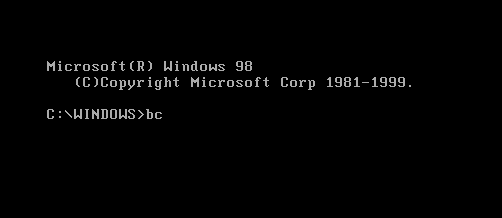
\includegraphics[width=0.7\textwidth]{reports/AC/lab2/assets/1.png}
    \caption{Запуск редактору Borland C}
\end{figure}

\begin{figure}[h]
    \centering
    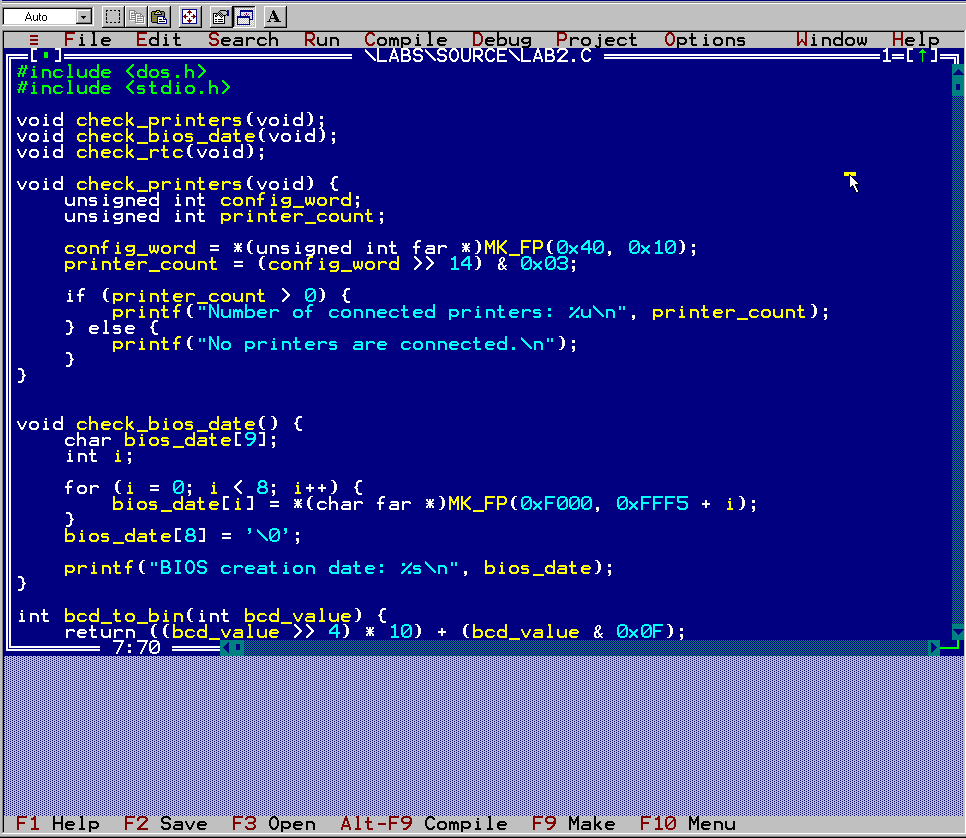
\includegraphics[width=0.8\textwidth]{reports/AC/lab2/assets/3.png}
    \caption{Запуск редактору Borland C}
\end{figure}

\begin{figure}[h]
    \centering
    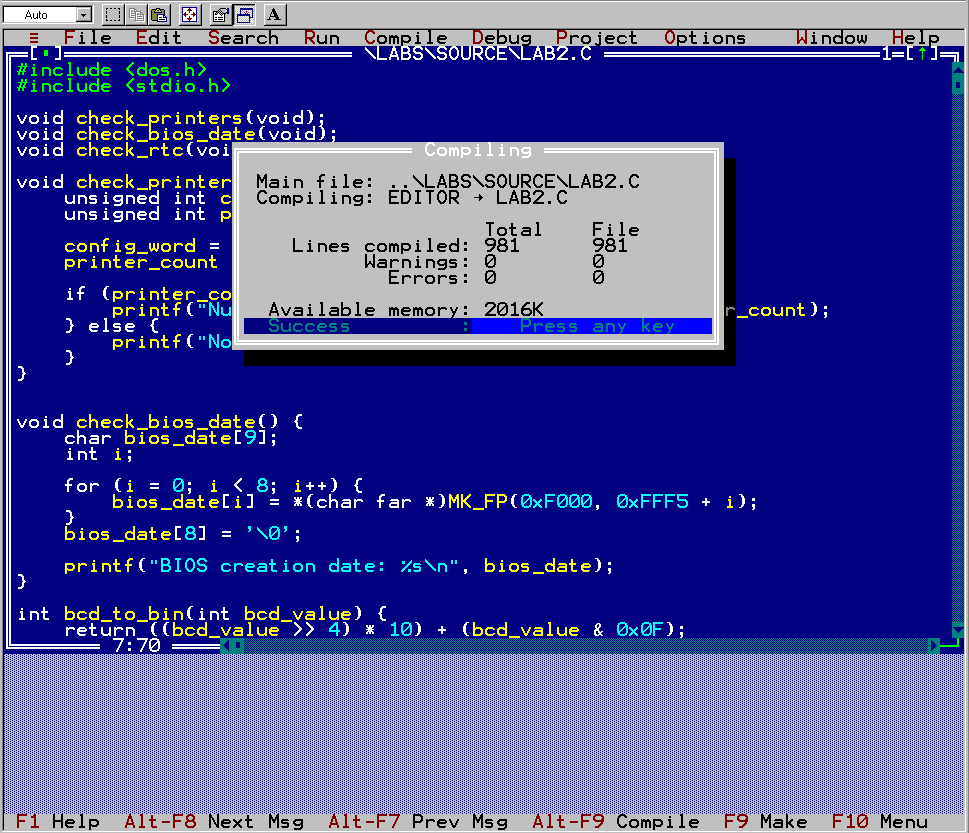
\includegraphics[width=0.9\textwidth]{reports/AC/lab2/assets/2.png}
    \caption{Успішна компіляція програми}
\end{figure}

\begin{figure}[h]
    \centering
    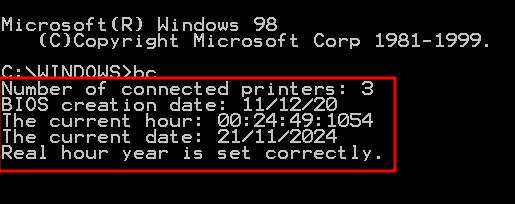
\includegraphics[width=0.7\textwidth]{reports/AC/lab2/assets/4.png}
    \caption{Результат робити програми у консолі}
\end{figure}

\clearpage
\section{Висновки}
    Під час виконання лабораторної роботи, я отримав практичні навички визначення конфігурації та основних
характеристик моєї ПЕОМ використовуючи мову програмування С у середовищі Borland C.

    Після виконання
скрипту можна побачити що на екран вивелася кількість підключених принтерів (може працювати не дуже
корректно через те що запускається на віртуальній машині), дату створення BIOS та перевірено правильність встановлення годиннику реального часу.
